% This document is used for Daya Bay MACRO PMT pressure test report


\documentclass{beamer}
\usepackage{graphics}
\setbeamertemplate{navigation symbols}{}
\setbeamertemplate{footline}[page number]
\setbeamertemplate{caption}[numbered]
%\setbeamerfont{purisa}
\usetheme{default}
\logo{
\includegraphics[height=1cm]{Dyb_logo.png}}
\begin{document}
\title{Status of MACRO PMT pressure tests at SAB}
\author{Logan Lebanowski, Shih-Kai Lin}
\institute{University of Houston}
\date{Sep 9, 2010}

\begin{frame}
\begin{center}
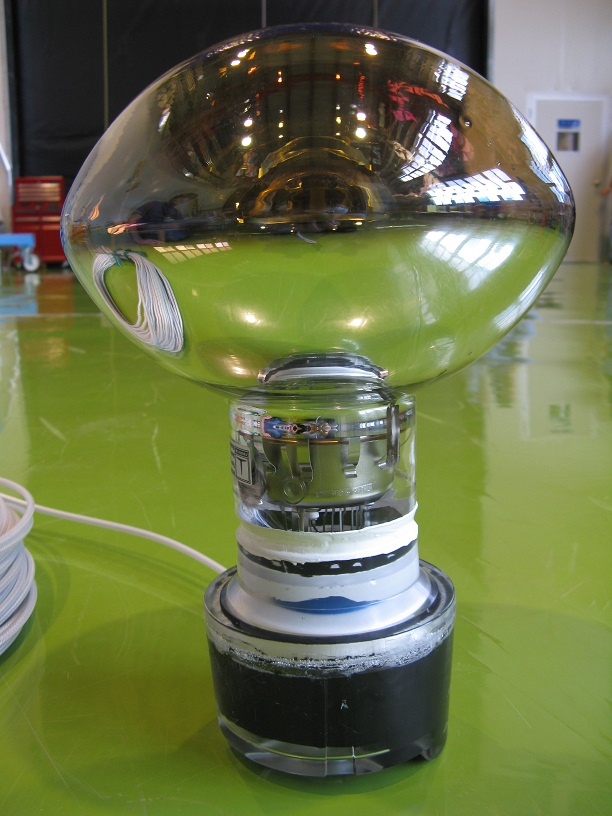
\includegraphics[height=4cm]{IMG_1048.jpg}
\end{center}
\titlepage
\end{frame}


\frame{\frametitle{Table of contents}\tableofcontents} 

\begin{frame}{pressure test result}
\begin{itemize}
 \item PMTs were tested during the past week (September 2 - September 8).
\end{itemize}
\begin{tabular}{c|c|c|c|c}
	SN & mass (g) & pressure (psig) & test time (h:m) & result \\
	\hline
	\hline
	7750 & 558.5 & 12.2 & 14:17 & 1 \\
	6297 & 619.5 & 12.1 & 8:55 & 2 \\
	8656 & 593 & 12.0 & 15:00 & 1 \\
	8459 & 553 & 12.2 & 8:13 & 1 \\
	7772 & 589 & 12.2 & 14:49 & 1 \\
	8932 & 630 & 12.2 & 47:49 & 1 \\
\end{tabular}
\end{frame}


\frame{\frametitle{lists with pause}
\begin{itemize}
\item Introduction to  \LaTeX \pause 
\item Course 2 \pause 
\item Termpapers and presentations with \LaTeX \pause 
\item Beamer class
\end{itemize} 
}

\frame{\frametitle{numbered lists with pause}
\begin{enumerate}
\item Introduction to  \LaTeX \pause 
\item Course 2 \pause 
\item Termpapers and presentations with \LaTeX \pause 
\item Beamer class
\end{enumerate}
}

\section{Section no.3} 
\subsection{Tables}
\frame{\frametitle{Tables}
\begin{tabular}{|c|c|c|}
\hline
\textbf{Date} & \textbf{Instructor} & \textbf{Title} \\
\hline
WS 04/05 & Sascha Frank & First steps with  \LaTeX  \\
\hline
SS 05 & Sascha Frank & \LaTeX \ Course serial \\
\hline
\end{tabular}}


\end{document}

